\PassOptionsToPackage{unicode=true}{hyperref} % options for packages loaded elsewhere
\PassOptionsToPackage{hyphens}{url}
%
\documentclass[]{article}
\usepackage{lmodern}
\usepackage{amssymb,amsmath}
\usepackage{ifxetex,ifluatex}
\usepackage{fixltx2e} % provides \textsubscript
\ifnum 0\ifxetex 1\fi\ifluatex 1\fi=0 % if pdftex
  \usepackage[T1]{fontenc}
  \usepackage[utf8]{inputenc}
  \usepackage{textcomp} % provides euro and other symbols
\else % if luatex or xelatex
  \usepackage{unicode-math}
  \defaultfontfeatures{Ligatures=TeX,Scale=MatchLowercase}
\fi
% use upquote if available, for straight quotes in verbatim environments
\IfFileExists{upquote.sty}{\usepackage{upquote}}{}
% use microtype if available
\IfFileExists{microtype.sty}{%
\usepackage[]{microtype}
\UseMicrotypeSet[protrusion]{basicmath} % disable protrusion for tt fonts
}{}
\IfFileExists{parskip.sty}{%
\usepackage{parskip}
}{% else
\setlength{\parindent}{0pt}
\setlength{\parskip}{6pt plus 2pt minus 1pt}
}
\usepackage{hyperref}
\hypersetup{
            pdftitle={Systematic review and climate change analysis in Los Lagos Region},
            pdfauthor={Derek Corcoran},
            pdfborder={0 0 0},
            breaklinks=true}
\urlstyle{same}  % don't use monospace font for urls
\usepackage[margin=1in]{geometry}
\usepackage{longtable,booktabs}
% Fix footnotes in tables (requires footnote package)
\IfFileExists{footnote.sty}{\usepackage{footnote}\makesavenoteenv{longtable}}{}
\usepackage{graphicx,grffile}
\makeatletter
\def\maxwidth{\ifdim\Gin@nat@width>\linewidth\linewidth\else\Gin@nat@width\fi}
\def\maxheight{\ifdim\Gin@nat@height>\textheight\textheight\else\Gin@nat@height\fi}
\makeatother
% Scale images if necessary, so that they will not overflow the page
% margins by default, and it is still possible to overwrite the defaults
% using explicit options in \includegraphics[width, height, ...]{}
\setkeys{Gin}{width=\maxwidth,height=\maxheight,keepaspectratio}
\setlength{\emergencystretch}{3em}  % prevent overfull lines
\providecommand{\tightlist}{%
  \setlength{\itemsep}{0pt}\setlength{\parskip}{0pt}}
\setcounter{secnumdepth}{5}
% Redefines (sub)paragraphs to behave more like sections
\ifx\paragraph\undefined\else
\let\oldparagraph\paragraph
\renewcommand{\paragraph}[1]{\oldparagraph{#1}\mbox{}}
\fi
\ifx\subparagraph\undefined\else
\let\oldsubparagraph\subparagraph
\renewcommand{\subparagraph}[1]{\oldsubparagraph{#1}\mbox{}}
\fi

% set default figure placement to htbp
\makeatletter
\def\fps@figure{htbp}
\makeatother

\usepackage{booktabs}
\usepackage{longtable}
\usepackage{array}
\usepackage{multirow}
\usepackage{wrapfig}
\usepackage{float}
\usepackage{colortbl}
\usepackage{pdflscape}
\usepackage{tabu}
\usepackage{threeparttable}
\usepackage{threeparttablex}
\usepackage[normalem]{ulem}
\usepackage{makecell}
\usepackage{xcolor}
\usepackage[]{natbib}
\bibliographystyle{plainnat}

\title{Systematic review and climate change analysis in Los Lagos Region}
\author{Derek Corcoran}
\date{2020-11-29}

\begin{document}
\maketitle

\hypertarget{climate-change-analisis}{%
\section{Climate change analisis}\label{climate-change-analisis}}

\hypertarget{climate-change-in-southern-chile}{%
\subsection{Climate change in southern Chile}\label{climate-change-in-southern-chile}}

In order to evaluate possible scenarios of climate change in the given area, we used a polygon comprising the Los Lagos and Los Ríos regions in Chile, and compared them using GCM compareR \citep{fajardo2020gcm}, considering Mean Anual Temperature and Annual Precipitation. The resulting scaled table of comparisson among futures was then use to select models to be used in the project.

We used the simple structure index (ssi) as implemented by the Vegan package \citep{Oksanen_2019, dolnicar1999tale} to test what number of clusters (Between two and eight), was the best way to represent the 32 Compared GCMs. The best representation was five clusters, from each cluster the GCM closest to the centroid of the cluster was selected. The five selected GCMS were cesm1\_bgc, gfdl\_esm2g, ipsl\_cm5a\_lr, miroc\_esm\_chem and mpi\_esm\_lr and the selected GCMs together with the clusters are shown in figure \ref{fig:SelectedGCMs}.

\begin{figure}
\centering
\includegraphics{Review_and_climate_files/figure-latex/SelectedGCMs-1.pdf}
\caption{\label{fig:SelectedGCMs}In this graph we can see the scaled temperature and precipitation axis, the center of the graph represent the ensemble of all models, the five groups represent the clusters selected using kmeans for five groups, the selected GCM of each cluster is shown with a label}
\end{figure}

\hypertarget{present-climate-conditions}{%
\subsubsection{Present climate conditions}\label{present-climate-conditions}}

Once the future GCM models were selected, the 30 seconds resolution maps were downloaded for 2070 and for present conditons from CHELSA \citep{karger2020high}.
The present conditions for the Los Lagos and Los Ríos Region are shown in Figure \ref{fig:PresenteClima}, with a close up to the 10 Km buffer surrounding the park in \ref{fig:PresenteClimaBuffer}. The region is a cold and humid area, with a range in the mean annual temperature from -5.6 to 13 degrees Celsius and a mean of 9.34, and a precipitation range between 858 to 4,537 and a mean of 2,092 mm a year.

\begin{figure}
\includegraphics[width=1\linewidth,height=1\textheight]{Review_and_climate_files/figure-latex/PresenteClima-1} \caption{Mean anual temperature in °C (Facet A), and Annual Precipitation mm (Facet B)}\label{fig:PresenteClima}
\end{figure}

The parks concidered in this proyect are in high altitude which leads to even cooler and wetter conditions, with a range from -5.6 to 12.6 and a mean of 8.12 degrees Celsius, and a precipitation range from from 1,176 to 3,410 and a mean of 2,134.51 mm as seen in figure \ref{fig:PresenteClimaBuffer}.

\begin{figure}
\includegraphics[width=1\linewidth,height=1\textheight]{Review_and_climate_files/figure-latex/PresenteClimaBuffer-1} \caption{Mean anual temperature in °C (Facet A), and Annual Precipitation mm (Facet B) in the three studied national parks white lines, and a 10 km buffer red line}\label{fig:PresenteClimaBuffer}
\end{figure}

\hypertarget{future-scenarios}{%
\subsection{Future scenarios}\label{future-scenarios}}

\hypertarget{future-temperature}{%
\subsubsection{Future temperature}\label{future-temperature}}

\begin{figure}
\centering
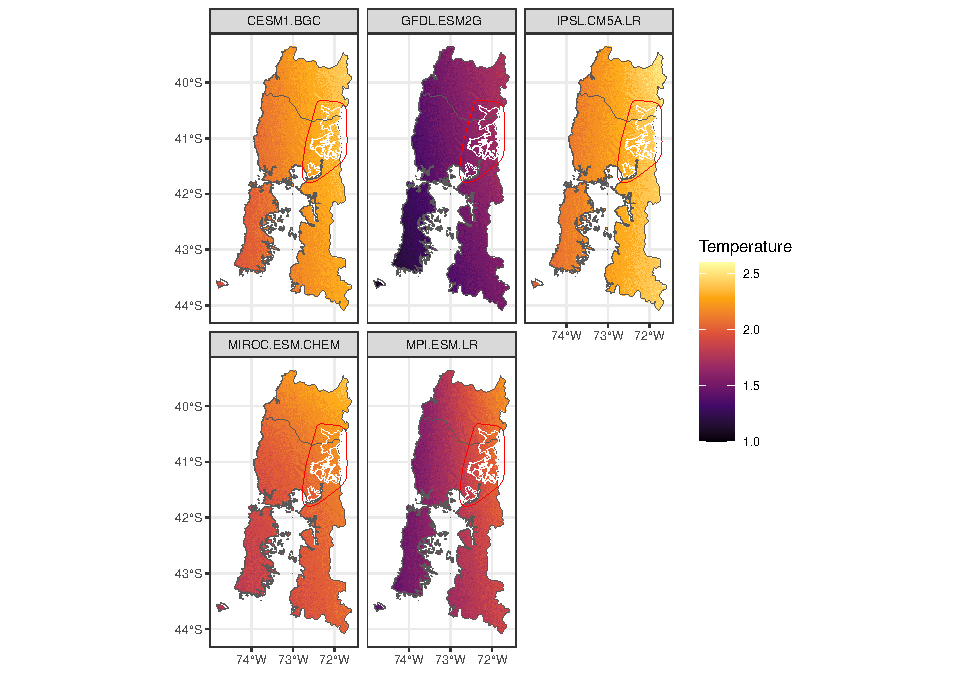
\includegraphics{Review_and_climate_files/figure-latex/DifTemp-1.pdf}
\caption{\label{fig:DifTemp}Changes in future mean annual temperature for the five selected GCMs, the red polygon surrounds the area of influence while the white line demarks the limits of the three protected areas in this proyect}
\end{figure}

As stated above, the four GCMs chosen to explore and model future scenarios are cesm1\_bgc, gfdl\_esm2g, ipsl\_cm5a\_lr, miroc\_esm\_chem and mpi\_esm\_lr. Even when this models include relatively wetter models such as cesm1\_bgc. On average for the whole region, the temperature will rise from 1.5 to 2.28 depending on the GCM (See figure \ref{fig:DifTemp}), but in some areas, it the tempearture rise could be as high as 2.6 degrees Celsius.

As seen in figure \ref{fig:DifTempHull}, those changes are even higher within the parks and it's sorrounding areas, which means the effects of climate change might be even greater.

\begin{figure}
\centering
\includegraphics{Review_and_climate_files/figure-latex/DifTempHull-1.pdf}
\caption{\label{fig:DifTempHull}Temperature difference for all five GCMs, for the Close up of the area of influence of the parks}
\end{figure}

\hypertarget{future-precipitation}{%
\subsubsection{Future precipitation}\label{future-precipitation}}

The change in precipitation is predicted to be much more stark, with some areas decreasing in precipitation up to -696 as seen in figure \ref{fig:DifPrec}, this is particularly worrisome, since the ecosystems that are prevalent in the area depend on high precipitation.

\begin{figure}
\centering
\includegraphics{Review_and_climate_files/figure-latex/DifPrec-1.pdf}
\caption{\label{fig:DifPrec}Changes in precipitation for the different GCMs, the red polygon surrounds the area of influence while the white line demarks the limits of the three protected areas in this proyect}
\end{figure}

\begin{figure}
\centering
\includegraphics{Review_and_climate_files/figure-latex/DifPrecHull-1.pdf}
\caption{\label{fig:DifPrecHull}Precipitation difference for all five GCMs, for the Close up of the area of influence of the parks}
\end{figure}

The range of changes between GCMs will be from from -376.99 to -313.23 mean annual precipitation for the whole area. Again the areas where there is going to be a higher drop in precipitation are mostly inside of the national parks, as seen in figure \ref{fig:DifPrecHull}, with changes in the mean annual precipitation within the are of -412.29 for the wettest models, and -320.96 for the driest models.

\renewcommand\refname{Vegetational formation}
\bibliography{Biblio.bib}

\end{document}
